\documentclass[11pt]{amsart}
\usepackage{geometry}                % See geometry.pdf to learn the layout options. There are lots.
\geometry{a4paper}                   % ... or a4paper or a5paper or ... 
%\geometry{landscape}                % Activate for for rotated page geometry
%\usepackage[parfill]{parskip}    % Activate to begin paragraphs with an empty line rather than an indent
\usepackage{graphicx}
\usepackage{amssymb, amsmath, amsthm}
\usepackage{natbib}
\usepackage{epstopdf}
\usepackage{enumerate}
\usepackage{textcomp}
\usepackage{mathrsfs }
\usepackage[section]{algorithm}
\usepackage{algorithmic}
\usepackage{tikz}
\usepackage{pgfplots}
\usepgfplotslibrary{patchplots}
%\usepackage{subfigure}
\usepackage{subcaption}

\usepackage{hyperref}
\usepackage{comment}
\usepackage{multirow}

%line suggested by my compiler (Fabian)
\pgfplotsset{compat=1.9}

% put figures at the end of the document, while I am writing is very annoying to have the figures in the middle of the text! 
% \usepackage[nomarkers,figuresonly]{endfloat}


\DeclareGraphicsRule{.tif}{png}{.png}{`convert #1 `dirname #1`/`basename #1 .tif`.png}

% \theoremstyle{theorem}
\newtheorem{theorem}{Theorem}[section]
\newtheorem{lemma}[theorem]{Lemma}
\newtheorem{proposition}[theorem]{Proposition}
\newtheorem{corollary}[theorem]{Corollary}
\newtheorem{point}[theorem]{}
\newtheorem{assumption}[theorem]{Assumption}


\theoremstyle{definition}
\newtheorem{definition}[theorem]{Definition}
\newtheorem{example}[theorem]{Example}
\newtheorem{notation}[theorem]{Notation}
\newtheorem{remark}[theorem]{Remark}
\newtheorem{condition}{Condition}

\newcommand{\F}{\operatorname{\mathcal{F}}}
\newcommand{\iF}{\operatorname{\mathcal{F}^{-1}}}

\newcommand{\Loperator}{\mathcal{L}}
%\newcommand{\R}{\mathbf{R}}
\newcommand{\Z}{\mathbf{Z}}

\newcommand{\dd}{\, \textrm{d}}
\newcommand{\e}{\textrm{exp}}
\newcommand{\fFrequency}{ f_{\omega_0}}
\newcommand{\fQuadrature}{ f_{\Delta}}

\newcommand{\I}{\mathbf{I}}

\newcommand{\ErrorFrequency}{\mathcal{E_F}}
\newcommand{\ErrorQuadrature}{\mathcal{E_Q}}
\newcommand{\Error}{\mathcal{E}}
\newcommand{\EF}{\ErrorFrequency}
\newcommand{\EQ}{\ErrorQuadrature}
\newcommand{\E}{\Error}
\newcommand{\est}{\overline {\mathcal{E}}}
\newcommand{\estFrequency}{\est_F}
\newcommand{\estQuadrature}{\est_Q}


\newcommand{\lx}{\mathcal{L}^{X}}
\newcommand{\ls}{\mathcal{L}^{S}}
\newcommand{\R}{\mathbb{R}}
\newcommand{\C}{\mathbb{C}}
\newcommand{\prob}[2]{\pi_{{#1,#2}}}
\newcommand{\lam}[1]{\lambda_#1}
\newcommand{\trials}[2]{\theta_{#1,#2}}
\newcommand{\damp}{\alpha}

\newcommand{\cgmyY}{Y}
\newcommand{\cgmyM}{\eta_+}
\newcommand{\cgmyG}{\eta_-}
\newcommand{\cgmyC}{K}

\newcommand{\cgmyexp}{\cgmyY}

\newcommand{\fa}{f_{\damp}}
\newcommand{\fadisc}[1]{f_{\damp, #1}}
\newcommand{\fdisc}[1]{f_{#1}}
\newcommand{\ga}{g_{\damp}}
\newcommand{\ha}{h_{\damp}}
\newcommand{\ft}[1]{\hat{#1}}
\newcommand{\kft}[1]{\tilde{#1}}
\newcommand{\ift}[1]{\iF\left[#1\right]}
\newcommand{\Lnorm}{\textrm{L}}
\newcommand{\real}[1]{\mathrm{Re}\left[#1\right]}
\newcommand{\im}[1]{\mathrm{Im}\left[#1\right]}
\newcommand{\step}{\Delta\omega}
\newcommand{\strip}[1]{A_{#1}}
\newcommand{\pureJumpProcessConstant}{C(\nu)}
\newcommand{\ffreq}[1]{\nu_{#1}}


\newcommand{\charExp}[1]{\Psi \parent{{#1}}}
\newcommand{\charFun}[2]{\varphi_{#1} \parent{{#2}}}

\newcommand{\cutoff}{\omega_{\mathrm{\max}}}
\newcommand{\strike}{k}

\newcommand{\pprob}[1]{}

\newcommand{\fnka}{f_{\damp}^{N,\cutoff}}
\newcommand{\ftnka}{\tilde f_{\damp}^{N,\cutoff}}

\newcommand{\pnka}{\Pi_{\damp}^{N,\cutoff}}

\newcommand{\fft}[2]{\mathrm{FFT}_{{#1}} \parent{{#2} }}
\newcommand{\tol}{\epsilon_{\mathrm T}}

\newcommand{\cutoffFrequency}{\omega_{\textrm{max}}}

\newcommand{\uremark}[2]{\underbrace{{#1}}_{{#2}}}

% Juho macros
\newcommand{\partder}[2]{\frac{\partial #1}{\partial #2}}
\newcommand{\der}[1]{\partial_{ #1}}
\newcommand{\ket}[1]{\left | {#1} \right \rangle }
\newcommand{\refstate}[0]{\textbf{0}}
\newcommand{\vacket}[0]{\ket{\refstate}}
\newcommand{\vacbra}[0]{\bra{\refstate}}
\newcommand{\bra}[1]{\left \langle {#1} \right | }
\newcommand{\ketbra}[1]{\ket{#1} \bra{#1}}
\newcommand{\innerprod}[2]{\left \langle {{#1} | {#2}} \right \rangle}
\newcommand{\uket}[0]{\ket{\uparrow}}
\newcommand{\dket}[0]{\ket{\downarrow}}
\newcommand{\ubra}[0]{\bra{\uparrow}}
\newcommand{\dbra}[0]{\bra{\downarrow}}
\newcommand{\hadj}[1]{{#1}^{\dagger}}
\newcommand{\conj}[1]{{#1}^{\ast}}
\newcommand{\cosine}[1]{\mathrm{cos}\left ( {#1}\right )}
\newcommand{\sine}[1]{\mathrm{sin}\left ( {#1}\right )}
\newcommand{\cosinep}[2]{\mathrm{cos}^{#2}\left ( {#1}\right )}
\newcommand{\sinep}[2]{\mathrm{sin}^{#2}\left ( {#1}\right )}
\newcommand{\expf}[1]{\mathrm{exp}\left ( {#1}\right )}
\newcommand{\expfs}[1]{e^{#1}}
\newcommand{\determinant}[1]{\mathrm{det}\left ( {#1}\right )}
\newcommand{\trace}[1]{\mathrm{Tr}\left ( {#1}\right )}
\newcommand{\parent}[1]{\left( {#1} \right)}
\newcommand{\aver}[1]{ \left\langle  {#1}  \right\rangle }
\newcommand{\absval}[1]{\left| {#1} \right|}
\newcommand{\sset}[1]{\left\lbrace {#1} \right\rbrace }
\newcommand{\iden}[1]{\mathbf{1}_{#1}}
\newcommand{\ssum}[2]{\displaystyle\sum\limits_{#1}^{#2}}
\newcommand{\pprod}[2]{\displaystyle\prod\limits_{#1}^{#2}}
\newcommand{\commut}[2]{\left[ {#1} , {#2} \right]}
\newcommand{\acommut}[2]{\left\lbrace  {#1} , {#2} \right\rbrace }
\newcommand{\spann}[1]{\mathrm{span} \parent{{#1}}}
\newcommand{\ttrace}[2]{\mathrm{Tr}_{#1} \parent{#2}}
\newcommand{\logt}[1]{\mathrm{log_2} \parent{{#1}}}
\newcommand{\hilbert}[1]{\mathcal{H}_{{#1}}}
\newcommand{\genus}{g}
\newcommand{\gsfun}[0]{\eta_{GS}}
\newcommand{\vvec}[1]{\textbf{{#1}}}
\newcommand{\kk}[0]{\vvec{k}}
\newcommand{\tsection}[1]{\newpage \section{{#1}}}
\newcommand{\grad}[0]{\nabla}
\newcommand{\divv}[0]{\nabla \dot}
\newcommand{\curl}[0]{\nabla \times}
\newcommand{\vvar}[1]{\mathrm{var} \parent{{#1}}}
\newcommand{\bigo}[1]{\mathcal O \parent{{#1}}}
\newcommand{\smallo}[1]{ o \parent{{#1}}}
\def\d{\textrm{d}}

\newcommand{\cost}[1]{C_{\mathrm{#1}}}

\newcommand{\qt}[0]{\tilde q}
%\newcommand{\e}[1]{\times 10^{#1}}
\newcommand{\supremum}[1]{\mathop{\mathrm{sup}}_{{#1}}}
\newcommand{\nnorm}[2]{\absval{\absval{{#1}}}_{#2}}
\newcommand{\problem}[1]{\newpage \section*{{#1}}}
\newcommand{\hittime}[0]{\sigma_{\bar{\mathcal E}}}
\newcommand{\probb}[1]{\mathrm{P} \parent{{#1}}}
\newcommand{\expp}[1]{\mathrm{E} \parent{{#1}}}

\newcommand{\kaustaddress}[0]{King Abdullah University of Science and Technology, Thuwal, Kingdom of Saudi Arabia}
\newcommand{\indicatorfun}[3]{\mathbf{1}_{[{#1},{#2}]} \parent{{#3}}}
\newcommand{\indicator}{\mathbf{1}}
\newcommand{\binaryg}[1]{g_{\mathrm{bin}} \parent{#1}}
\newcommand{\binaryf}[1]{f_{\mathrm{bin}} \parent{#1}}
\newcommand{\fbinaryf}[1]{\hat{f}_{\mathrm{bin}} \parent{#1}}

\newcommand{\callg}[1]{g_{\mathrm{call}} \parent{#1}}
\newcommand{\fcallg}[1]{\hat{g}_{\mathrm{call}} \parent{#1}}
\newcommand{\fcallga}[1]{\hat{g}_{\mathrm{call}, \damp} \parent{#1}}
\newcommand{\fputga}[1]{\hat{g}_{\mathrm{put}, \damp} \parent{#1}}
\newcommand{\fcallf}[1]{\hat{f}_{\mathrm{call}} \parent{#1}}
\newcommand{\fcallfa}[1]{\hat{f}_{\mathrm{call}, \damp} \parent{#1}}


\newcommand{\evaldiff}[3]{{\left [ {#1} \right ]}_{#2}^{#3}} 

\newcommand{\vga}{a}
\newcommand{\vgb}{b}

\newcommand{\vgpoly}[1]{w  \parent{#1}}
\newcommand{\vgaux}{q}

\newcommand{\imo}{y}
\newcommand{\reo}{x}
\newcommand{\abex}{\rho}

%%% for the merton case
\newcommand{\sj}{\sigma_{\mathrm{jump}}}
\newcommand{\rj}{r_{\mathrm{jump}}}


%% I always forget the correct spelling
\newcommand{\levy}{L\'evy }
\newcommand{\levynospace}{L\'evy}
%%

\newcommand{\rz}{\R \setminus \sset{0}}

\newcommand{\linf}[1]{L^\infty_{#1}}
\newcommand{\norminf}[2]{\left\|#1\right\|_{\linf{#2}}}
\newcommand{\cl}{C \parent{\lambda}}

\pgfmathdeclarefunction{lg10}{1}{%
    \pgfmathparse{ln(#1)/ln(10)}%
}


\title[MIMC and MLMC HJM]{Multi-Index and Multi-Level Monte Carlo Evaluation of HJM Models}
\author{Juho H\"app\"ol\"a}
\address{\kaustaddress}
\email{juho.happola@iki.fi}


\date{\today}    
                                    % Activate to display a given date or no date
\begin{document}


\begin{abstract}
Notes of MIMC and MLMC evaluation of HJM models.
\end{abstract}

\maketitle
%\tableofcontents

\section{Intro}

We are interested in analysing the Forward Euler Finite Difference evaluation of forward curve models of HJM models. The main approach was represented with a convergence analysis in \cite{bjork2013monte}, whose notation we largely follow.

We are focused on the evolution of the forward curve $f \parent{t , \tau}$ for $t \in [0,t_{max}]$, $\tau \in [0,\tau_{max}]$ with $\tau_{max}>t_{max}$. In order to define a mesh for the numerical solution of the problem, let us define $\bar \ell \in \mathbb{N}^3$.

Let our quantity of interest be defined as the expectation of a functional $\mathcal F$
of the forward curve:
\begin{align*}
\mathcal F \parent f =& F \parent{\int_0 ^{t_{max}} f \parent{s,s} ds}
G \parent{ \int_{\tau_a}^{\tau_{max}} \Psi \parent{f \parent{t_{max},\tau}} d\tau }
\\
&+
\int_{0}^{t_{max}} F \parent{\int_0^{s} f \parent{s',s'} ds'} U \parent{f\parent{s,s}} ds.
\end{align*}

Let us first discretise the time interval as
\begin{align*}
\Delta t_{\bar \ell} &= 2^{-\ell_1} t_{max},
\\
t_{\bar \ell, n} &= n \Delta t_{\bar \ell}, ~~~ n \in [0,1,2,\cdots, 2^{\ell_1}].
\end{align*}
Since there is an additional requirement that $t_{max}$ be in
the mesh of maturities, one point in the mesh in $\tau \in [0,\tau_{max}]$. We let $\ell_1$ and $\ell_2$ define the number of discretisation points to the right and to the left of the fixed
point, respectively.
\begin{align*}
\Delta \tau_{\bar \ell,1} &= 2^{-\ell_3} t_{max},  \\
\Delta \tau_{\bar \ell,2} &= 2^{-\ell_2} \parent{\tau_{max}-t_{max}}, \\
\tau_{\bar \ell, n} &= n \Delta \tau t_{\bar \ell,1}, ~~~ n \in [0,1,2,\cdots, 2^{\ell_3}] \\
\tau_{\bar \ell, n} &= n \Delta \tau t_{\bar \ell,1}, ~~~ n \in [2^{\ell_3},2^{\ell_3}+1,\cdots, 2^{\ell_3}+2^{\ell 2}].
\end{align*}

Using this notation, we have the following rates of convergence, following the Multi-Index notation:
\begin{align}
\bar \beta &= [2,2,2]^T \\
\bar \gamma &= [1,1,1]^T .
\end{align} 
Choosing the Simpson method for integration, we have the order of quadrature $p_Q=3$, which brings the quadrature error to 
\begin{align}
\expp{\absval{\mathcal G\parent{\bar{\bar g}} - \mathcal G \parent{g}}^{2 \kappa}} \leq C \parent{\Delta \tau_{\bar \ell}}^{2 \kappa p_Q} = 
\tilde C 2^{-6 \kappa \mathrm{min} \parent{\ell_3,\ell_2}}.
\end{align}
On the other hand, the error of the simpson method is the sum of errors for $\tau < t_{max}$ and $\tau \leq t_{max}$. The error for these two domains are $\bigo{2^{-2 \ell_2}}$ and $\bigo {2^{-2 \ell_3}}$, respectively. Combining together, we get the weak and the strong rate
for the Simpson quadrature:
\begin{align}
\expp{\absval{\mathcal G\parent{\bar{\bar g}} - \mathcal G \parent{g}}^{2}} \leq&  \tilde C_Q 2^{-6 \mathrm{min} \parent{\ell_3,\ell_2}}
\\
\expp{\absval{\mathcal G\parent{\bar{\bar g}} - \mathcal G \parent{g}}} \leq& C_Q 2^{-2 \mathrm{min} \parent{\ell_2,\ell_3}}.
\end{align}

\begin{align}
\expp{\absval{\mathcal G\parent{\bar{\bar g}} - \mathcal G \parent{g}}^{2 \kappa}}
\end{align}
using Theorem 3.3 of \cite{bjork2013monte}.

On the other hand, theorem 3.2 and equation (3.54) states that
\begin{align}
\expp{ \absval{ \mathcal G \parent{g} - \mathcal G \parent{\bar{\bar g}} }^{2 \kappa}  } ^{\frac{1}{2 \kappa}} \leq C_{5}^{CV} \parent{ \parent{\Delta t}^{\frac{1}{2}} + \Delta \tau }.
\end{align}

The weak rate for the discretisation error can be bounded by eq. (4.6):
\begin{align}
\expp{ \absval{ \mathcal G \parent{g} - \mathcal G \parent{\bar{\bar g}} }^{}  }
= 
 \bigo{\parent{\Delta t}^2 + \parent{\Delta \tau}^2}
 = \bigo{2^{-2 \ell_1} + 2^{-2 \mathrm {min} \parent{\ell_2,\ell_3} }}
\end{align}

Due to the fact that the discretisation errors relating to $\tau$
depend on the minimum of $\ell_2$ and $\ell_3$, it seems natural
to assume $\ell_3=\ell_2$. This gives us a two-dimensional
Multi-Index Monte Carlo formulation with the following effective parameters
\begin{align}
\bar \beta &= [2,2]^T ,\\
\bar \gamma &= [1,1]^T , \\
\bar s &= [1,2], \\
\bar w & = [1,2].
\end{align}

On the other hand, one may set $\ell_1=\ell_2=\ell_3=\ell$
and arrive at a one-dimensional MLMC formulation with a weak rate of $2$, strong rate of $1$, and computational cost per realisation of $W_\ell=2^{2\ell}$. In the sequel, we will present the results of these two variations for comparison.

\section{Numerical tests}

For the simplest possible example, let our model be Gaussian with
the following exponential covariance structure
\begin{align}
\expp{df \parent{t,\tau} df \parent{t, \tau'}}
=
\sigma^2 \expf{- \kappa \absval{\tau-\tau'}} dt.
\end{align}

Let our first test case be arguably simplest infinite dimensional one possible,
\begin{align*}
F \parent{x} &= 1-x,\\
U \parent{x} &= 0, \\
G \parent{x} &= x, \\
\Psi \parent{x} &= x, \\
f \parent{0,\tau} &= 0, \\
\kappa &= 2.
\end{align*}

In \ref{fig:empInfDimRates} we get see that we have rate one for both 
the weak and the strong rate along both dimensions for this text example.

\begin{figure}
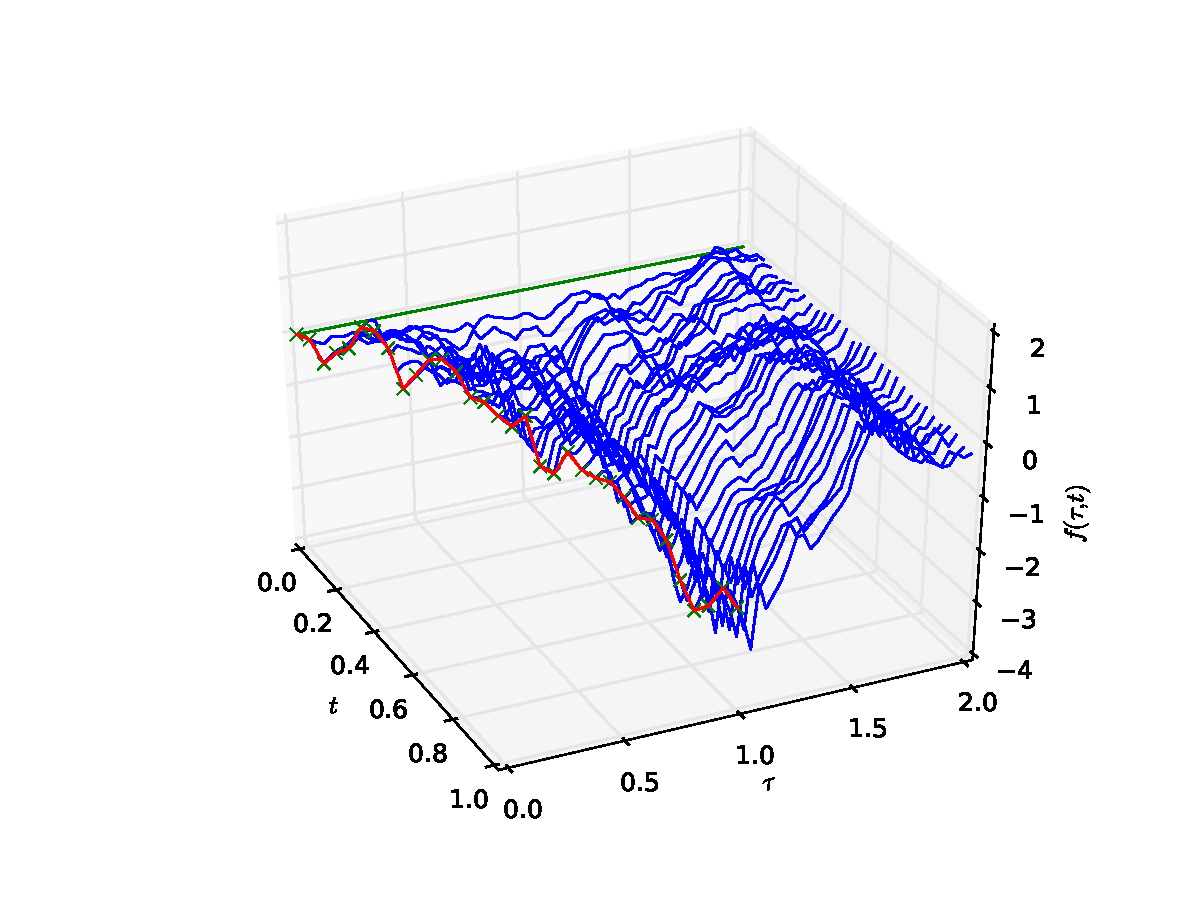
\includegraphics[scale=0.7]{figure_1.pdf}
\caption{Sample realisation of a forward curve with the discretisation level 
$\overline \ell = [5,5,5]^T$.}
\end{figure}

It remains to deduce the cost of simulating the cost of a realisation. In order to
simulate Gaussian random variables one needs the Cholesky decomposition of the covariance matrix. The cost to generate this $N_\tau \times N_\tau$-matrix is $N_\tau^3$, with $N_\tau = 2^{\ell_3} 2^{\ell_2}$. Using the Cholesky decomposition, the cost to take a a time step becomes $N_\tau^2$. Putting all together, the cost to generate $M$ Monte Carlo realisations with $N_t$ time steps and $N_\tau$ discretisation steps along the maturity direction becomes
\begin{align*}
C \parent{\Delta t, \Delta \tau, M} = N_\tau^3 + M N_\tau^2 N_t.
\end{align*}

\begin{figure}
    \centering
    \begin{subfigure}[b]{0.4\textwidth}
        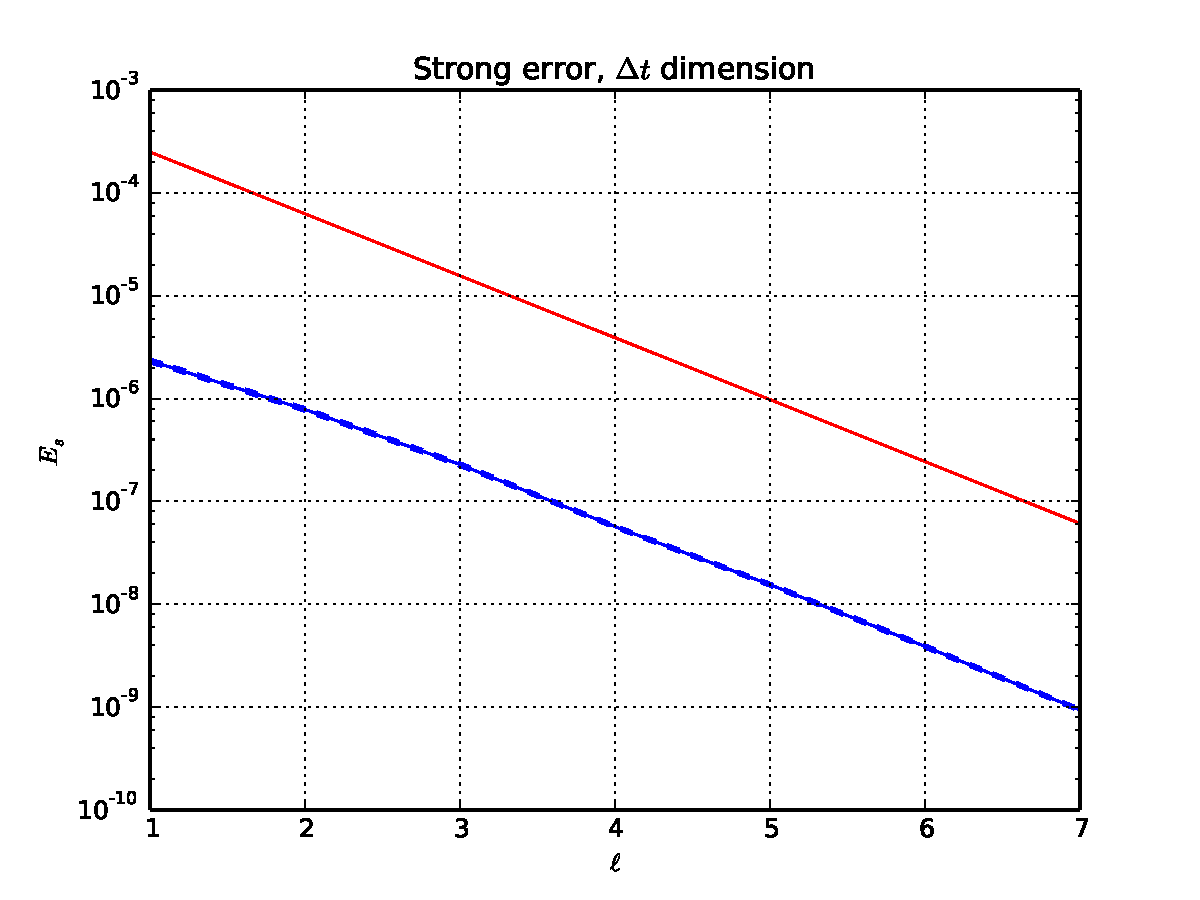
\includegraphics[width=\textwidth]{dim_1_strong.pdf}
        %\caption{A gull}
        \label{fig:gull}
    \end{subfigure}
    ~ %add desired spacing between images, e. g. ~, \quad, \qquad, \hfill etc. 
      %(or a blank line to force the subfigure onto a new line)
    \begin{subfigure}[b]{0.4\textwidth}
        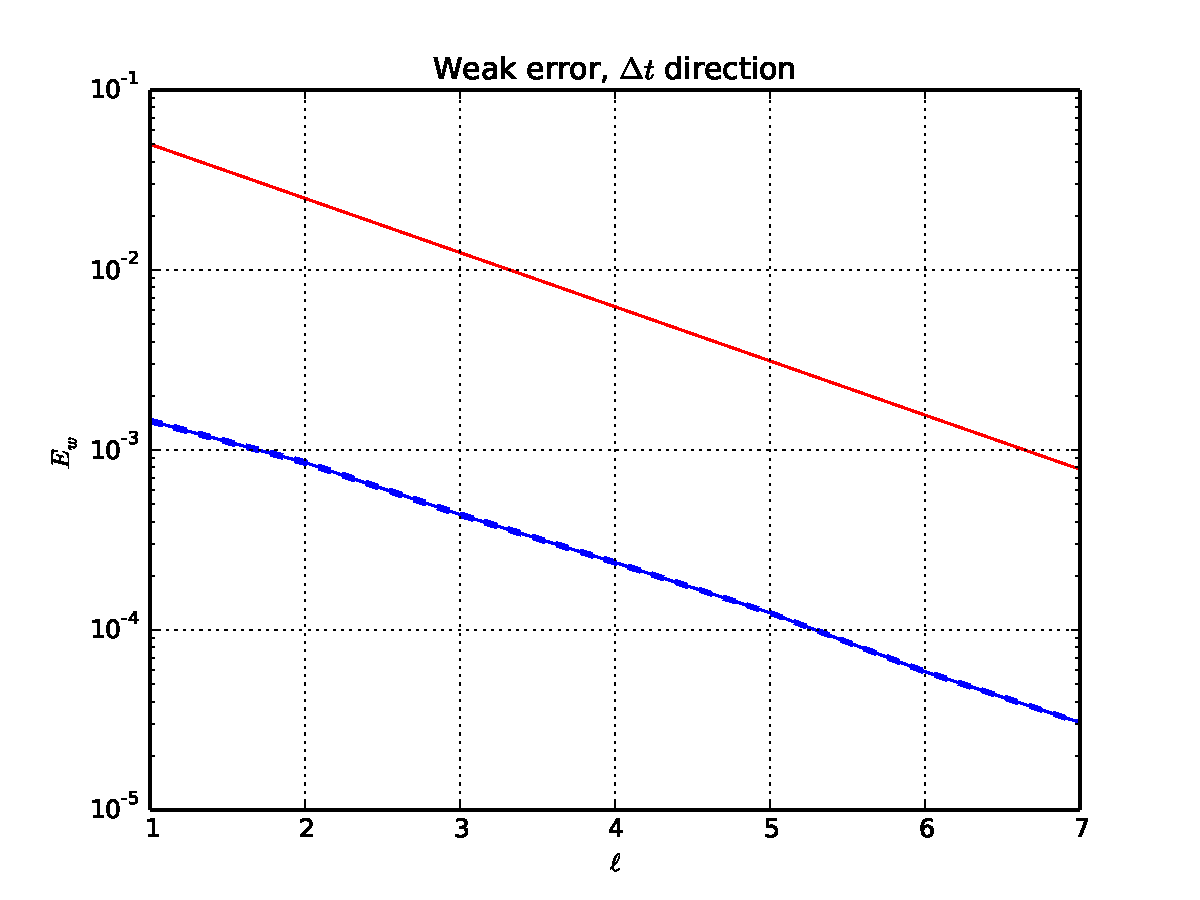
\includegraphics[width=\textwidth]{dim_1_weak.pdf}
        %\caption{A tiger}
        \label{fig:tiger}
    \end{subfigure}
    \\
    ~ %add desired spacing between images, e. g. ~, \quad, \qquad, \hfill etc. 
    %(or a blank line to force the subfigure onto a new line)
    \begin{subfigure}[b]{0.4\textwidth}
        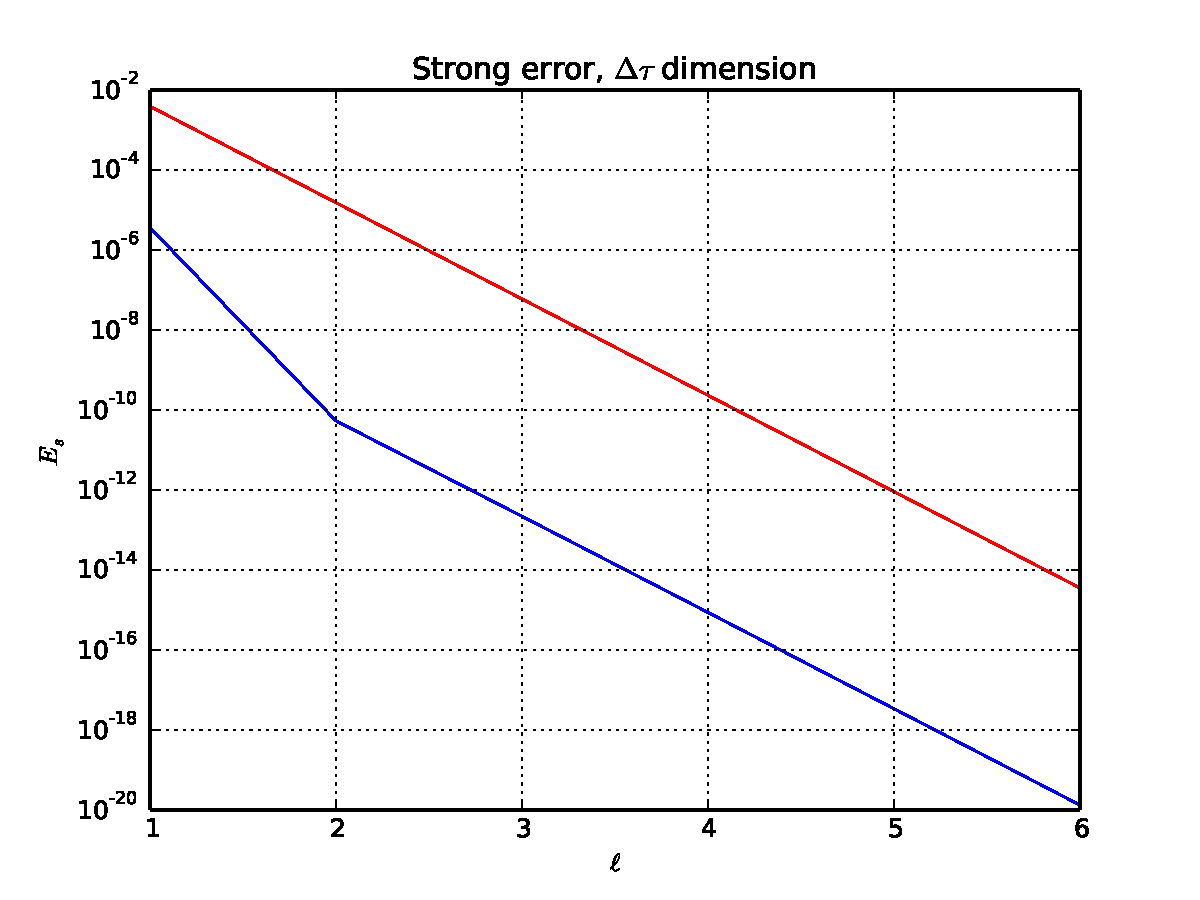
\includegraphics[width=\textwidth]{dim_2_strong.pdf}
        %\caption{A mouse}
        \label{fig:mouse}
    \end{subfigure}
        \begin{subfigure}[b]{0.4\textwidth}
        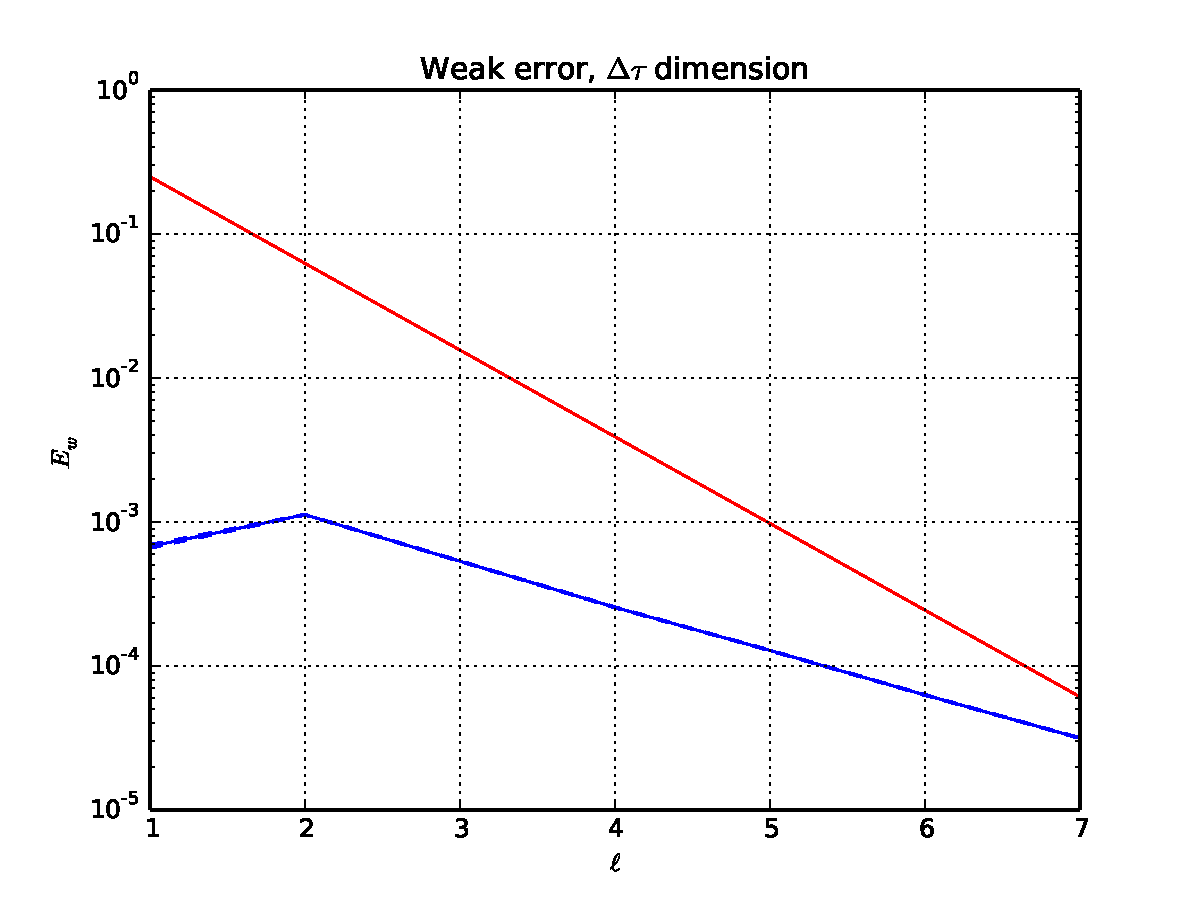
\includegraphics[width=\textwidth]{dim_2_weak.pdf}
        %\caption{A mouse}
        \label{fig:mouse}
    \end{subfigure}
    \caption{\label{fig:empInfDimRates}Empirical strong and weak convergence rate for the $\Delta t$ and $\Delta \tau$ discretisation errors.}
\end{figure}



\bibliographystyle{agsm}
\bibliography{references}

\appendix




\end{document}


